% effect of temperature on contrastive learning loss function & embedding space
The parameter $\tau$ is called temperature.
\citet{CL_temp_2021} have carried out an exhaustive study on the impact of temperature on the loss function of \ac{cl}.
% define hardness
They found that the contrastive loss function optimizes hard samples by penalizing them according to their hardness.
In the context of \ac{cl}, hardness refers to the difficulty associated with accurately classifying 
a sample as either positive or negative in relation to a given anchor.
Hard samples are those that pose significant challenges for the model: 
They may be hard positives, which are distant from the anchor yet from the same class, 
or hard negatives, which are misleadingly close to the anchor despite being from a different class.

\begin{figure}[!htb] % h = here, t = top, b = bottom, p = page of floats
    \centering
    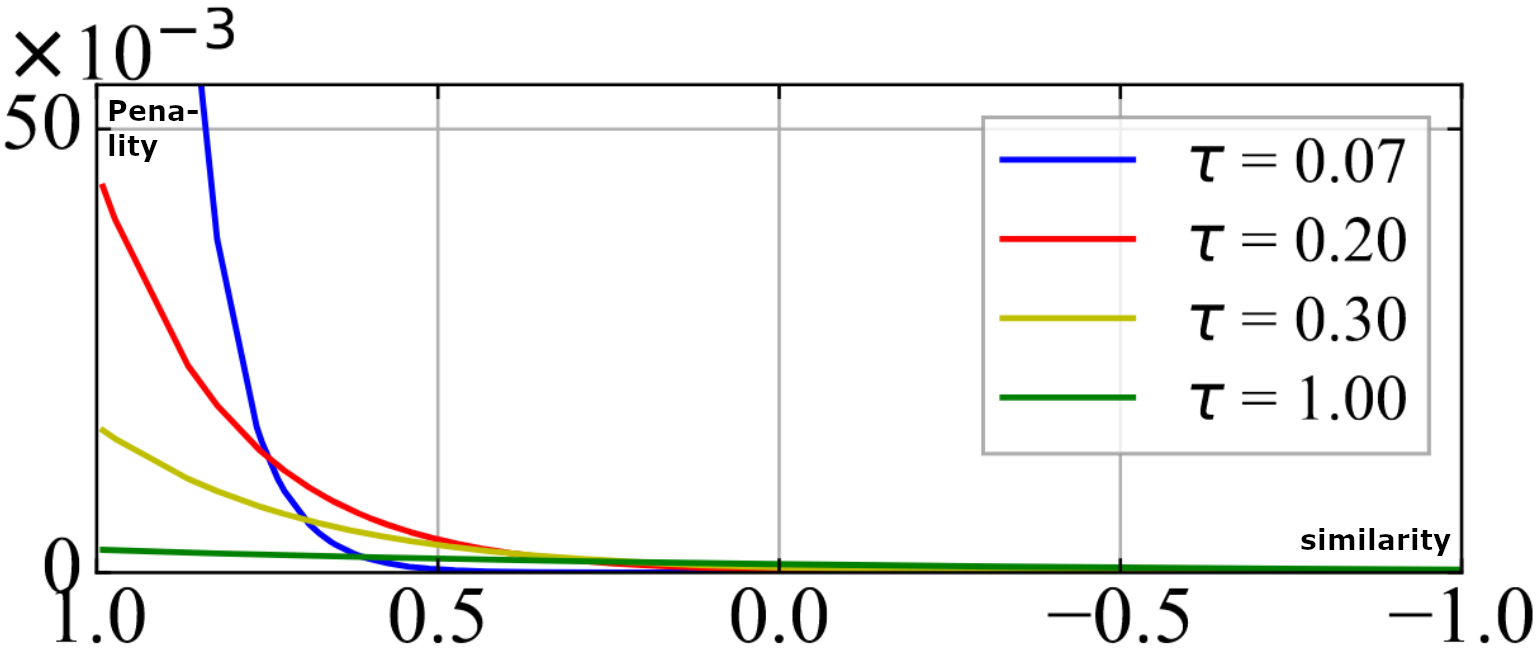
\includegraphics[width=280pt]{images/gradient_ratio_dep_on_temperature_legend.png}
    \caption{Penality (y-axis) depending on similarity of samples (x-axis) similar to \citet{CL_temp_2021}. 
    For small values of $\tau$, similar samples, i.e. x-axis values close to $1.0$, receive high penalties.
    If $\tau$ is too small, only the closest one or two points are penalized and thus, the performance deteriorates.
    As $\tau \rightarrow 1$, the magnitude of the penalty is similar for all negative samples.
    }
    \label{fig:gradient_ratio_dep_on_temperature}
\end{figure}

\begin{figure}[!htb] % h = here, t = top, b = bottom, p = page of floats
    \centering
    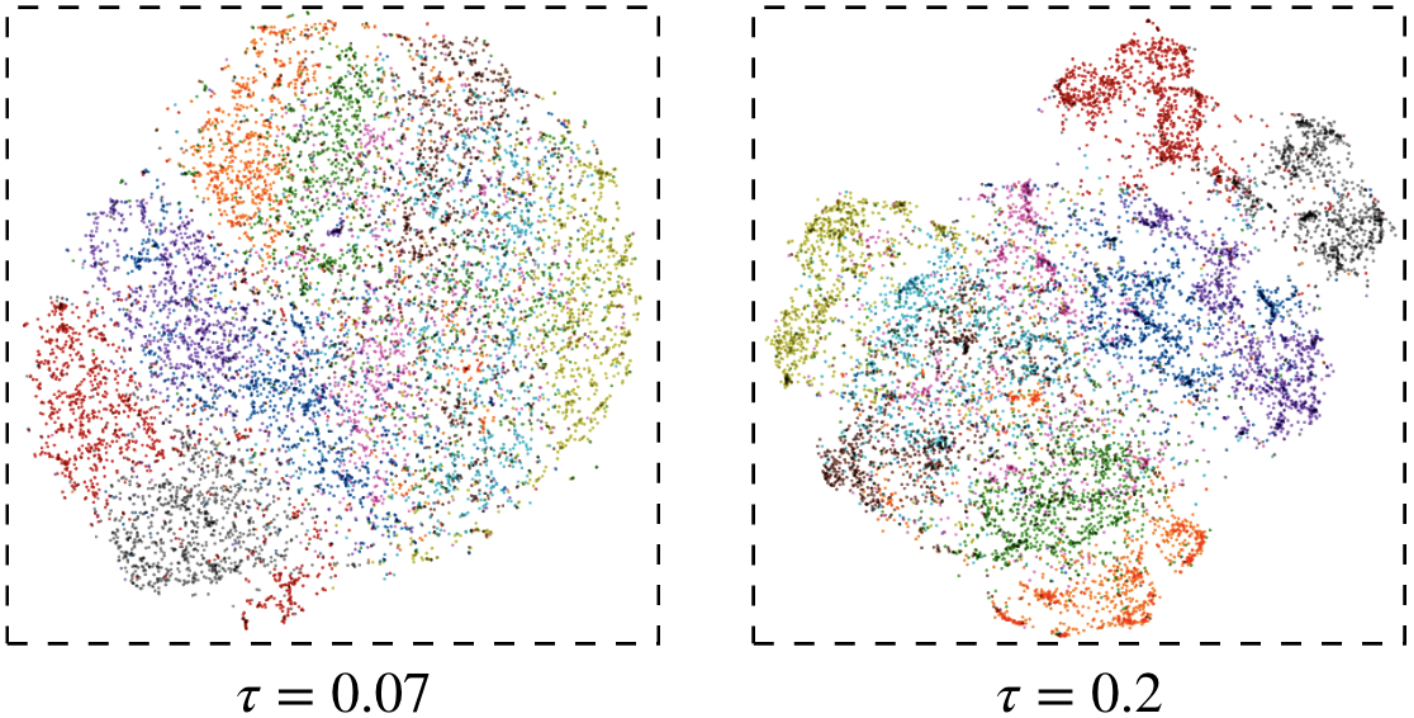
\includegraphics[width=280pt]{images/tsne_dep_on_temperature.png}
    \caption{Visualization of embedding space for different $\tau$ from \citet{CL_temp_2021}.
    Small values of $\tau$ lead to a more uniform distribution of the embedding space, 
    because similar samples are repelled.
    }
    \label{fig:tsne_dep_on_temperature}
\end{figure}

% impact of temperature
As displayed in \autoref{fig:gradient_ratio_dep_on_temperature}, 
small temperatures $\tau$ lead to a greater penalty for very hard negative samples, i.e. those that are similar to the anchor.
Consequently, the representations of these samples are pushed further apart, 
resulting in a more uniformly distributed embedding space \citep{CL_temp_2021,grape_2024}. 
This effect is further demonstrated in \autoref{fig:tsne_dep_on_temperature}.
However, when $\tau$ is too small, the embedding spaces' semantic structure deteriorates.
For $\tau \rightarrow \infty$, the loss function's hardness-aware property disappears and hard negatives are not penalized anymore.